%
% karteextremum.tex
%
% (c) 2021 Prof Dr Andreas Müller, OST Ostschweizer Fachhochschule
%
\documentclass[tikz]{standalone}
\usepackage{times}
\usepackage{amsmath}
\usepackage{txfonts}
\usepackage[utf8]{inputenc}
\usepackage{graphics}
\usetikzlibrary{arrows,intersections,math}
\usepackage{ifthen}
\begin{document}
\definecolor{darkred}{rgb}{0.8,0,0}

\newboolean{showgrid}
\setboolean{showgrid}{false}
\def\breite{7}
\def\hoehe{4}
\def\h{4.1}

\begin{tikzpicture}[>=latex,thick]

% Povray Bild
\begin{scope}
\clip (-6.3,-\h) rectangle (6.3,\h);
\node at (0,0) {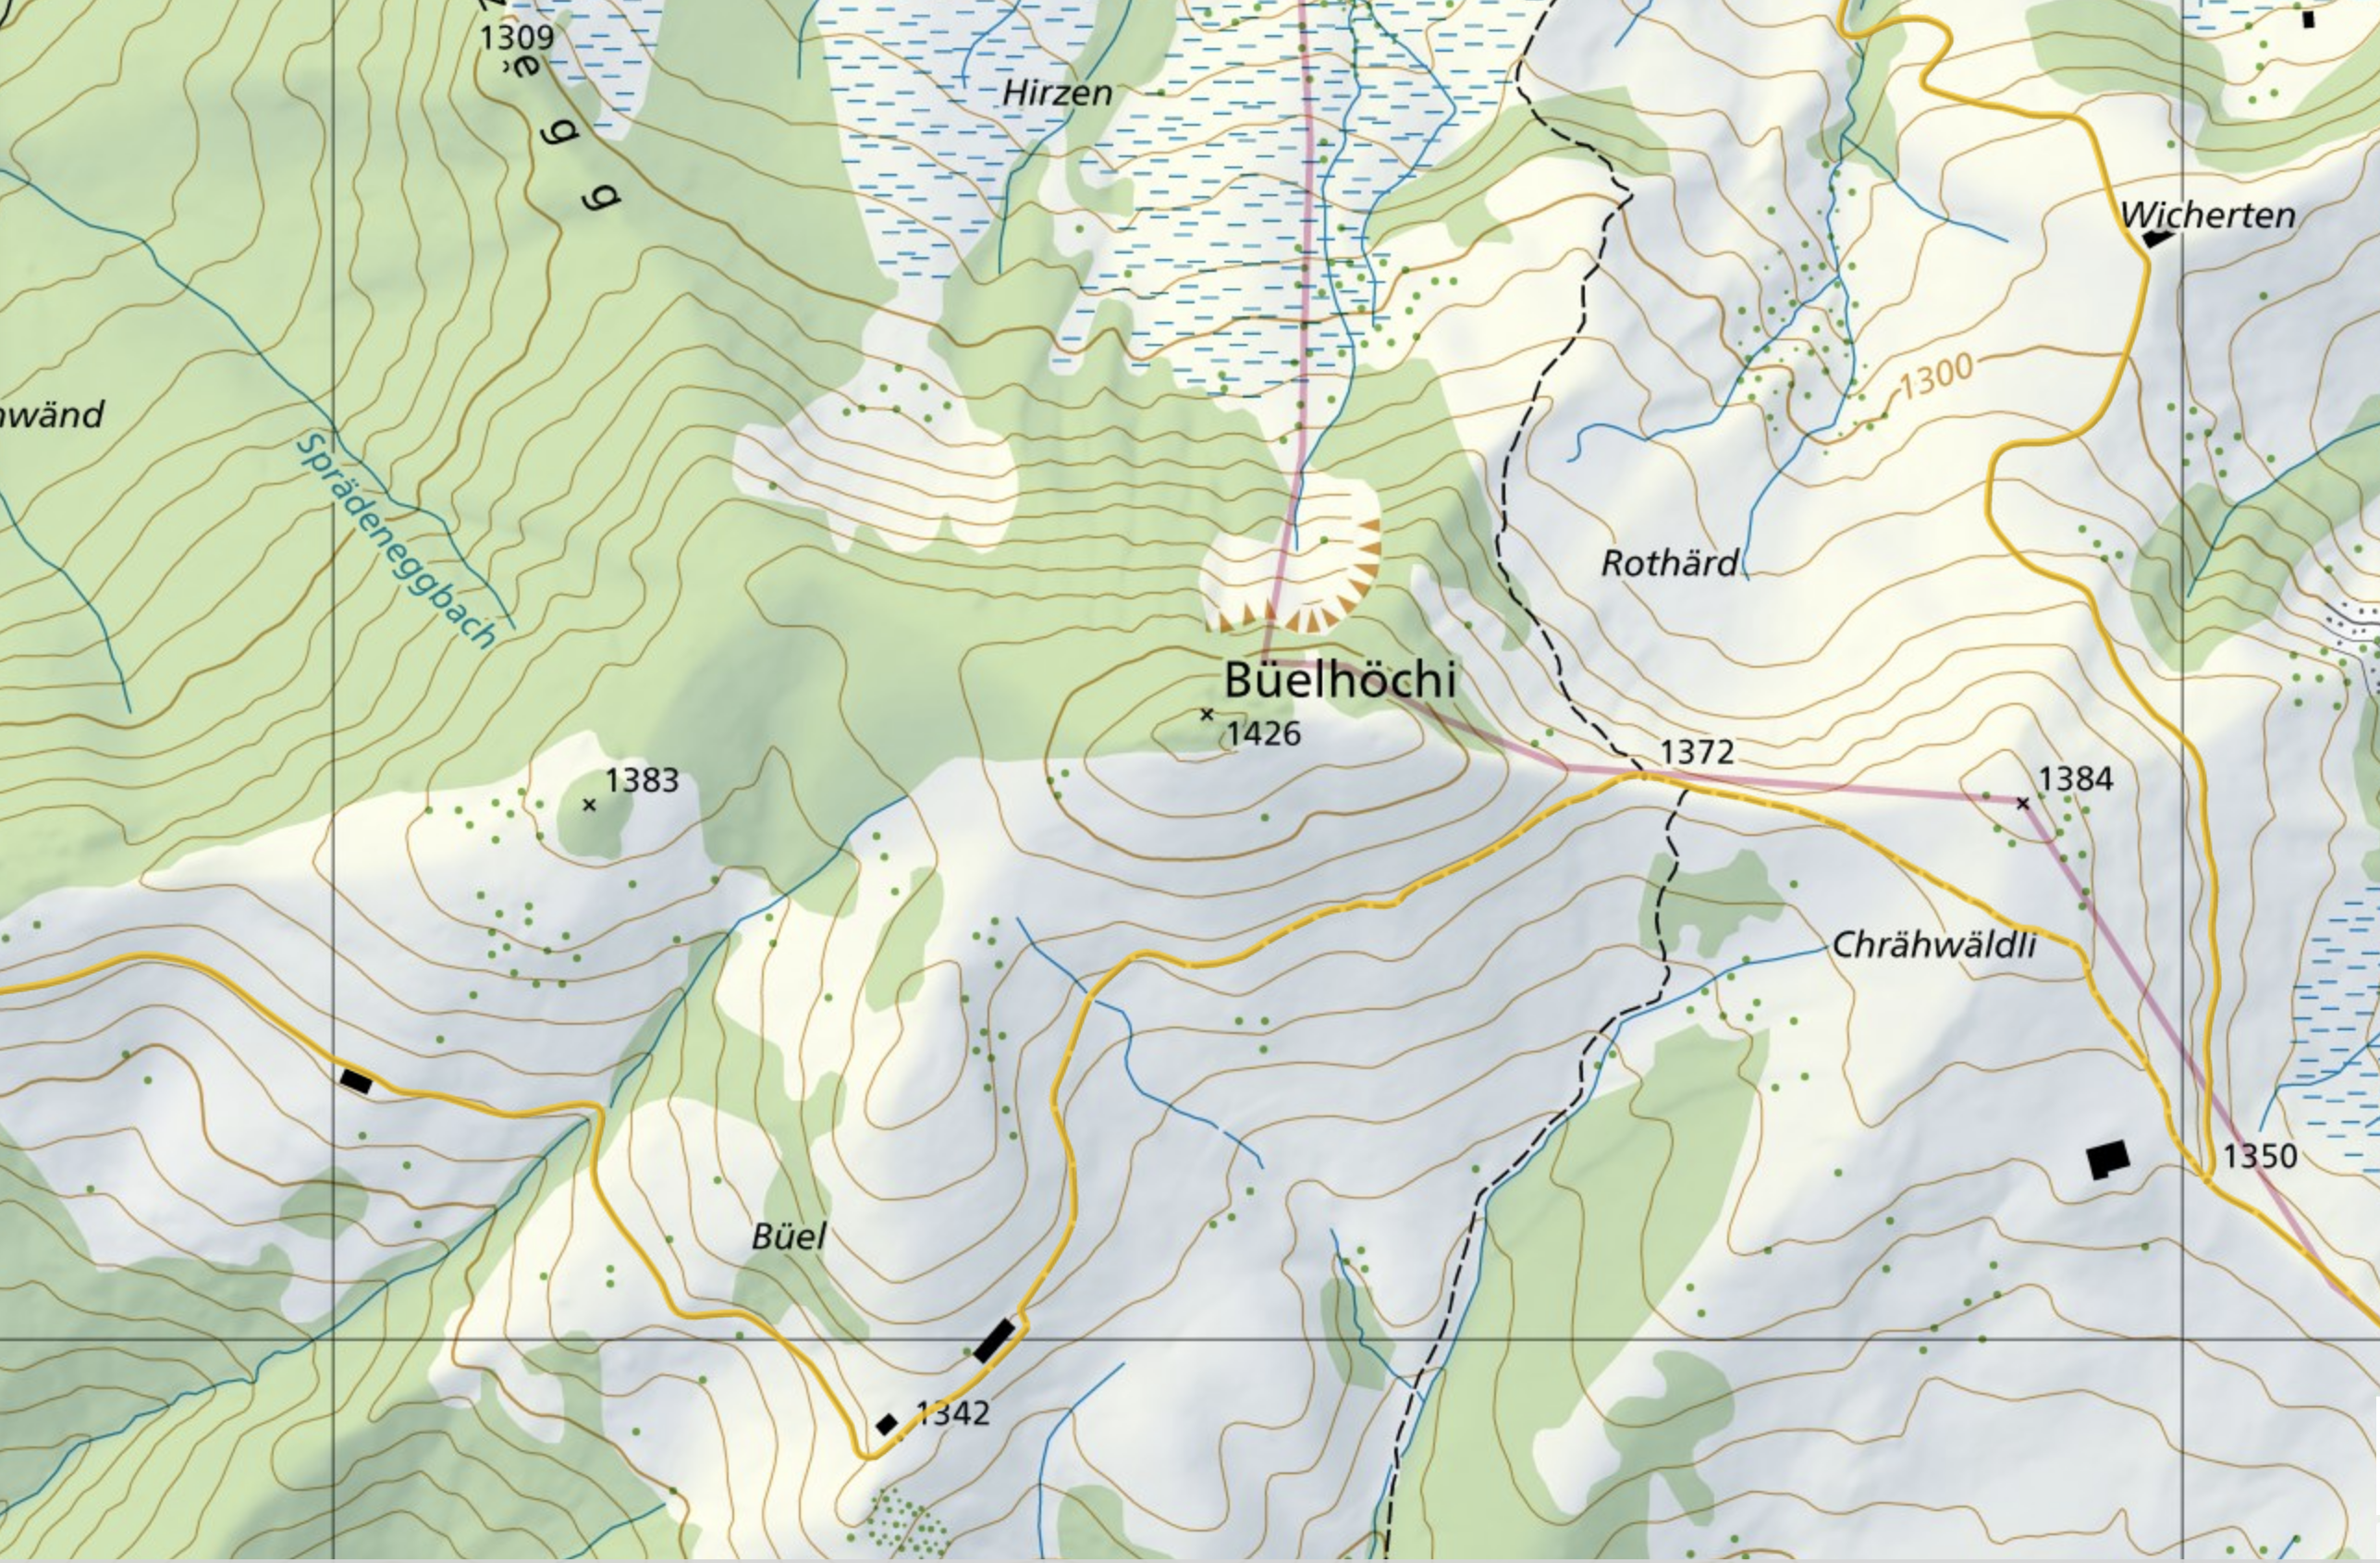
\includegraphics[width=12.6cm]{karte.png}};
\end{scope}

% Gitter
\ifthenelse{\boolean{showgrid}}{
\draw[step=0.1,line width=0.1pt] (-\breite,-\hoehe) grid (\breite, \hoehe);
\draw[step=0.5,line width=0.4pt] (-\breite,-\hoehe) grid (\breite, \hoehe);
\draw                            (-\breite,-\hoehe) grid (\breite, \hoehe);
\fill (0,0) circle[radius=0.05];
}{}

\draw[color=blue] (3.6,-0.32) circle[radius=0.08];
\draw[color=blue] (-4.37,-1.54) circle[radius=0.08];

\draw[color=darkred] (1.5,-0.42) circle[radius=0.08];
\draw[color=darkred] (-3.75,-1.74) circle[radius=0.08];
\draw[color=darkred] (-5.2,-0.99) circle[radius=0.08];

\end{tikzpicture}

\end{document}

